\begin{ex}
(Ufrs) A figura a seguir representa uma parede quadrada na qual estão pintados discos de raio r. Se uma bola é lançada totalmente ao acaso contra a parede, a probabilidade de ela tocar fora dos discos está entre:
\begin{center}
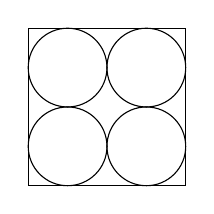
\begin{tikzpicture}
 \draw (.5,.5) circle [radius = .5];
 \draw (1.5,.5) circle [radius = .5];
 \draw (1.5,1.5) circle [radius = .5];
 \draw (.5,1.5) circle [radius = .5];
 \draw (0,0)--(2,0)--(2,2)--(0,2)--(0,0);
\end{tikzpicture}
\end{center}
   \begin{enumerate}[(a)]
   \item 14\% e 16\%
   \item 17\% e 19\%
   \item 20\% e 22\%
   \item 23\% e 25\%
   \item 26\% e 28\%
   \end{enumerate}
    \begin{sol}
     resposta: c \\
     $p=\frac{16r^2-4\pi r^2}{16r^2}=\frac{3,44}{16}=21,5\%$
    \end{sol}
\end{ex}